\documentclass[12pt]{article}
\usepackage{mymarco} % my marco file
\usepackage{parskip} % no auto indent
\usepackage[margin=1.0in]{geometry}
\usepackage{fancyhdr}
\pagestyle{fancy}
\setlength{\headheight}{15pt}
\rhead{Shawn Wu} % Define header
\lhead{Decay Rate Reverse Order}
\cfoot{\thepage}

\begin{document}
\underline{\textbf{Goal:}} Find an upper bound \(F(r)\) of the function,
\begin{align*}
    f(r) = \int_{\R^3} e^{-\alpha_1|\vr_1 - \vc_1| - \alpha_2|\vr_1 - \vc_2|-\alpha_3|\vr_1 + r\vomg - \vc_3|-\alpha_4|\vr_1 + r\vomg - \vc_4|} \diff \vr_1,
\end{align*}
such that \(f(r) \leq F(r) = \mathcal{O}(e^{-\beta r})\) for some \(\beta > 0\). And the bound should be easy to calculate with only elementary operations. Also the bound should be tight, since we are deciding at which point of \(r\) we can just chop off the rest, if the bound if not tight, it will not have numerical difference.

\underline{\textbf{Intuition:}} Note that the exponent in the integrand can be written as 
\begin{align*}
    -\alpha_1|\vr_1 - \vc_1| - \alpha_2|\vr_1 - \vc_2|-\alpha_3|\vr_1 - (\vc_3-r\vomg)|-\alpha_4|\vr_1 - (\vc_4 - r\vomg)|,
\end{align*} 
meaning that as \(r\) grows to infinity, we can think the centres \(\vc_3, \vc_4\) are moving away from \(\vc_1, \vc_2\) in the direction \(-\omega\) up to infinity. And the indefinie integral \(f(r)\) should goes to zero exponentially as \(r\) grows to infinity because when the molecues are too far apart, then electric replusion energy between them should disspate quickly.

\underline{\textbf{General Strategy:}} 
We analyze the case when the domain is 1D first, then 2D, then finally move on to 3D. 
Note that for any four points in \(\R^3\) (assuming the points are not coplanar), there are no points that would be "trapped" in-between other points, meaning that every point has "access" to any infinite amount of space (more precisely, if we construct the Voronoi diagram based on the four points, then each point would belong to a cell that has infinite volume).
To keep this property in its lower-dimensonal counterparts, we will have two centres in the 1D case, and three centres in 2D (assuming that the points are linearly independent).

Also note that the indefinite integral \(\int_{\R^n} e^{-\beta |\vr_1|} \diff \vr_1\) is rather easy to calulate in any dimensions,
\begin{align*}
    \int_{\R^n} e^{-\beta |\vr_1|} \diff \vr_1 = \frac{2 \pi^{n/2}\Gamma(n)}{\Gamma(n/2) \beta^n}. \tag{\(\ast\)}
\end{align*}
Therefore, the general strategy is to upper bound the \textit{integrand} with one \(\mu(r)e^{-\beta|\vr_1|}\) or several \(\mu_i(r)e^{-\beta_i|\vr_1|}\)'s pieced together where \(\mu(r) = \mathcal{O}(e^{-\gamma r})\) (\(\gamma > 0\)) so that
\begin{align*}
    f(r) 
    \leq 
    \underbrace{\int_{\R_n} \mu(r) e^{-\beta|\vr_1|} \diff \vr_1}_{F(r)}
    =
    \mu(r) \underbrace{\int_{\R_n}  e^{-\beta|\vr_1|} \diff \vr_1}_{\text{constant}}
    = \mathcal{O}(e^{-\gamma r})
\end{align*}

\textbf{\underline{Attempt 1} (only with triangluar inequality):} This unforunately doesn't work. The integral can be bounded by some function of the form \(\mu(r)e^{-\beta|\vx|}\) but \(\mu(r)\) doesn't decay exponentially as \(r\) grows. Let's see why in the 1D case. Suppose the direction vector \(\vomg = 1\). We have
\begin{align*}
    f(r) = \int_{\R} e^{-\alpha_1|r_1 - c_1| - \alpha_2 |r_1 - (c_2 - r)| } \dr_1.
\end{align*}
Then \(|r_1 - c_1| \geq |r_1| - |c_1|\) and \(|r_1 - (c_2 - r)| \geq |r_1| - |c_2 - r|\).
Therefore, the expoenet
\begin{align*}
    &-\alpha_1|r_1 - c_1| - \alpha_2 |r_1 - (c_2 - r)| \\
    \leq& -(\alpha_1 + \alpha_2)|r_1| + \alpha_1|c_1| + \alpha_2|c_2 - r|  \\
    \leq& -(\alpha_1 + \alpha_2)|r_1| + (\alpha_1|c_1| + \alpha_2|c_2|) + \alpha_2 r.
\end{align*}
Therefore,
\begin{align*}
    e^{-\alpha_1|r_1 - c_1| - \alpha_2 |r_1 - (c_2 - r)|} \leq e^{\alpha_2 r} \cdot e^{\alpha_1|c_1| + \alpha_2|c_2|}\cdot e^{-(\alpha_1 + \alpha_2)|r_1|},
\end{align*}
which gives
\begin{align*}
    \int_{\R}  e^{-\alpha_1|r_1 - c_1| - \alpha_2 |r_1 - (c_2 - r)|}
    \leq 
    \underbrace{e^{\alpha_2 r}}_{\mathcal{O}(e^{\alpha_2r})}
    \cdot 
    \overbrace{e^{\alpha_1|c_1| + \alpha_2|c_2|}}^{\text{constant}} 
    \underbrace{\int_{\R} e^{-(\alpha_1 + \alpha_2)|r_1|} \dr_1}_{\text{constant by }(\ast)}.
\end{align*}
However, this upper bound grows exponentially!

\textbf{\underline{Attempt 2} (slicing in 1D):} This actually works!
Suppose we have the following setup where \(\omega = -1, c_1 < c_2, r \geq 0\). And two STOs, \(\Phi_1(r_1) = \exp(-\alpha_1|r_1-c_1|), \Phi_2(r_1,r) = \exp(-\alpha_2|r_1 - (c_2 + r)|)\).
Then the integrand is \(\Psi(r_1,r) = \Phi_1(r_1) \Phi_2(r_1,r)\). 

\begin{center}
    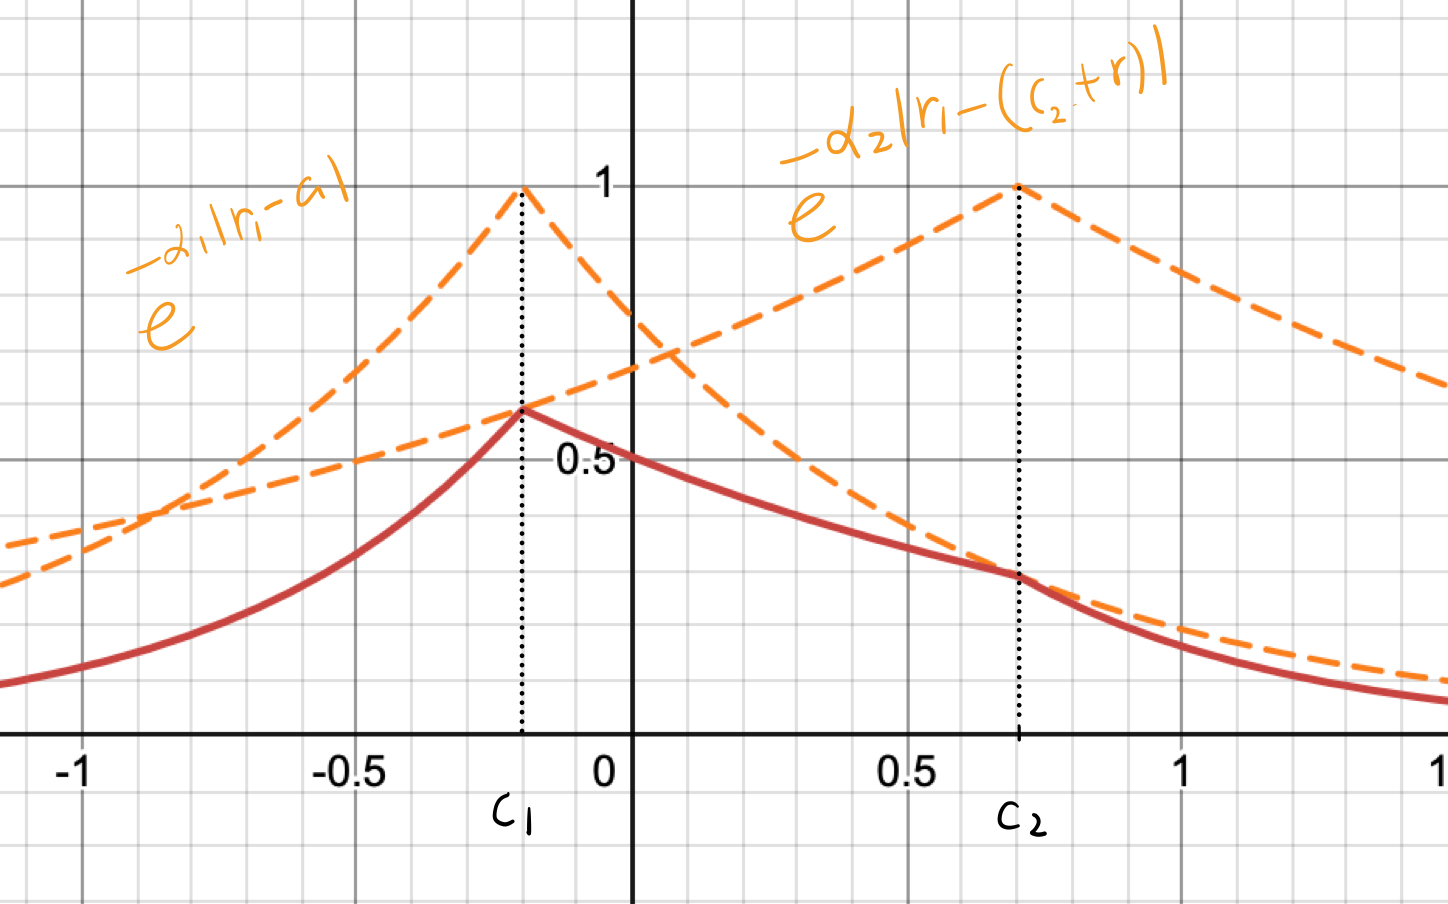
\includegraphics[scale=0.21]{figure1.jpeg}
\end{center}
Click \href{https://www.desmos.com/calculator/zuqivaujt4}{\underline{here}} to see the full graph.
We bound \(\Psi(r_1,r)\) piecewise. We claim that for fixed \(r\),
\begin{enumerate}
    \item on \((-\infty, c_1]\), \(\Psi(r_1,r) \leq \mu_1(r) \cdot \exp(-(\alpha_1 + \alpha_2)|r_1-c_1|)\), where \(\mu_1(r) = \Phi_2(c_1,r)\).
    \item on \([c_2,+\infty)\), \(\Psi(r_1,r) \leq \mu_2(r) \cdot \exp(-(\alpha_1 + \alpha_2)|r_1-c_2|)\), where \(\mu_2(r) = \Phi_1(c_2+r).\)
    \item on \([c_1,c_2]\), the line segement \(\ell\) between points \((c_1, \Psi(c_1,r))\) and \((c_2, \Psi(c_2,r))\),
\end{enumerate}
where it's clear that both \(\mu_1(r), \mu_2(r) = \mathcal{O}(e^{-\beta r})\) for some \(\beta > 0\).

We first note that the third claim is straightforward, as \(\Psi(r_1,r)\) between \(c_1,c_2\) is always convex proven by Prof. Kaur. We will thus only show the proof for the first claim as the second is similar.

\begin{proof}
Note that on the interval \((-\infty,c_1]\), \(   |r_1 - c_1| < |r_1 - (c_2+r)|\), so
\begin{align*} 
    & -\alpha_2 |r_1-c_1| > -\alpha_2|r_1-(c_2+r)|\\
    \implies & -\alpha_1|r_1-c_1| - \alpha_2|r_1-(c_2+r)| < -\alpha_1|r_1-c_1| - \alpha_2|r_1-c_1|\\
    \implies & -\alpha_1|r_1-c_1| - \alpha_2|r_1-(c_2+r)| < -(\alpha_1 + \alpha_2)|r_1 - c_1|\\
    \implies & \exp(-\alpha_1|r_1-c_1| - \alpha_2|r_1-(c_2+r)|) < \exp(-(\alpha_1 + \alpha_2)|r_1 - c_1|),
\end{align*}
which gives,
\begin{align*}
    \boxed{\Psi(r_1, r) \leq \exp(-(\alpha_1 + \alpha_2)|r_1-c_1|)} \tag{\(\ast\ast\)}
\end{align*}
Graphicaly, this upper bound is the following blue curve.
\begin{center}
    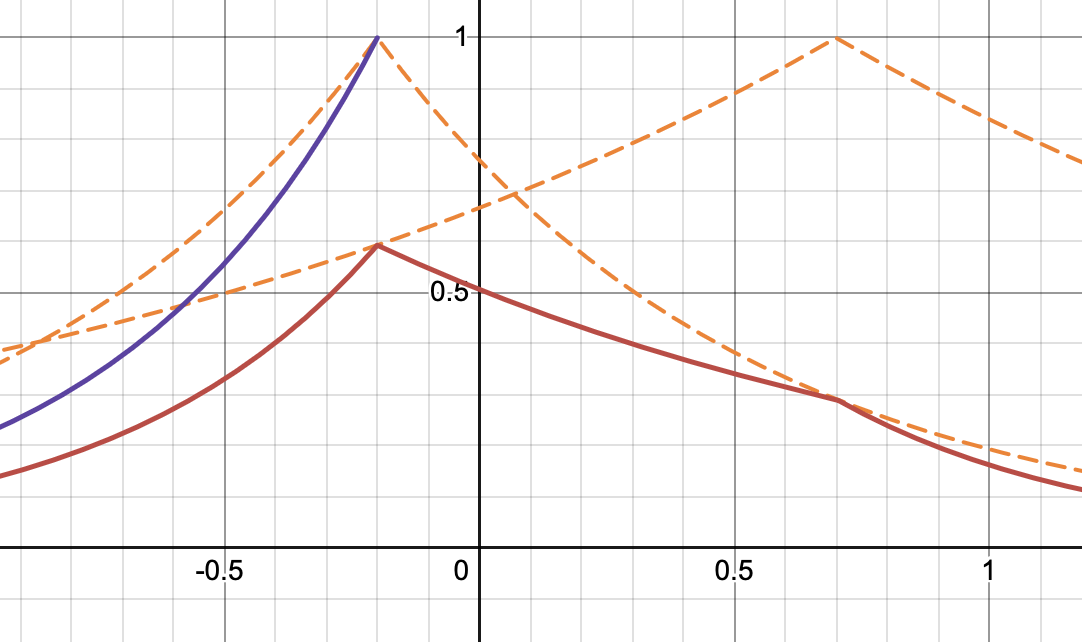
\includegraphics[scale=0.5]{figure2.png}
\end{center}
However, to make the upper bound decay exponentially as the function of \(r\), we need the coefficient term \(\mu_1(r)\) to decay fast, and in the case of 1D, \(\mu_1(r) = \Phi_2(c_1,r)\) will suffice.

Note that when \(r_1 < c_1\), \(|r_1 - (c_2+r)| = |r_1 - c_1| + |c_1 - (c_2+r)|\).
Therefore,
\begin{align*}
    &-\alpha_2|r_1 - (c_2+r)| = -\alpha_2|r_1 - c_1| -\alpha_2|c_1 - (c_2+r)|\\
    \implies & -\alpha_1|r_1-c_1|-\alpha_2|r_1 - (c_2+r)|= -\alpha_1|r_1-c_1|-\alpha_2|r_1 - c_1| -\alpha_2|c_1 - (c_2+r)|\\
    \implies & -\alpha_1|r_1-c_1|-\alpha_2|r_1 - (c_2+r)|= -(\alpha_1 + \alpha_2)|r_1 - c_1| -\alpha_2|c_1 - (c_2+r)|\\
    \implies & \exp(-\alpha_1|r_1-c_1|-\alpha_2|r_1 - (c_2+r)|) = \exp(-(\alpha_1 + \alpha_2)|r_1 - c_1| -\alpha_2|c_1 - (c_2+r)|)\\
    \implies &\exp(-\alpha_1|r_1-c_1|-\alpha_2|r_1 - (c_2+r)|) = \exp(-(\alpha_1 + \alpha_2)|r_1 - c_1|)\cdot \exp(-\alpha_2|c_1 - (c_2+r)|)\\
    \implies & \Psi(r_1,r) \leq \Phi_2(c_1,r) \cdot \exp(-(\alpha_1 + \alpha_2)|r_1 - c_1|),
\end{align*}
which gives a very tight bound (equality actually!) on \((-\infty, c_1]\) (showing up here as the dotted purple curve below).

\begin{center}
    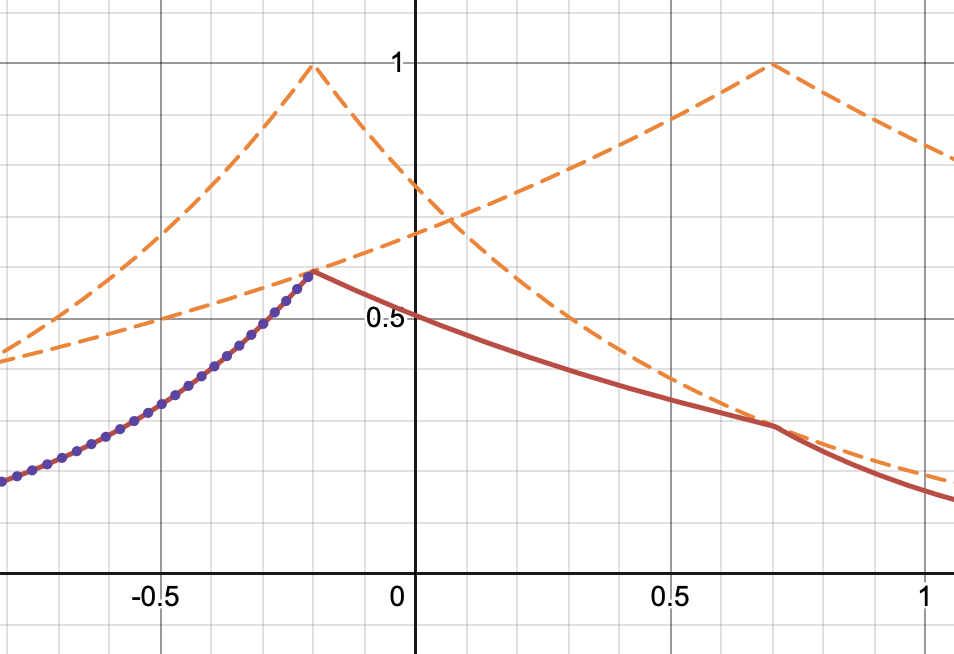
\includegraphics[scale=0.5]{figure3.png}
\end{center}

Therefore,
\begin{align*}
    \int_{\R} \Phi(r_1,r) \dr_1 \leq& \int_{(-\infty,c_1]} \mu_1(r) \exp(-(\alpha_1 + \alpha_2)|r_1 - c_1|) \dr_1
    + \int_{[c_1,c_2]} \ell \dr_1 \\
    +&\int_{[c_2,+\infty)} \mu_2(r) \exp(-(\alpha_1 + \alpha_2)|r_1 - c_2|) \dr_1.
\end{align*}
And let \(\alpha = \min(\alpha_1 , \alpha_2)\).

Therefore,
\begin{align*}
    \int_{(-\infty,c_1]} \mu_1(r) \exp(-(\alpha_1 + \alpha_2)|r_1 - c_1|) \dr_1 \
    &= \mu_1(r)\cdot \frac{1}{2} \overbrace{\int_{\R} \exp(-(\alpha_1 + \alpha_2)|r_1 - c_1|) \dr_1}^{2/(\alpha_1 + \alpha_2)}\\
    &= \frac{\Phi_2(c_1, r)}{\alpha_1 + \alpha_2}\\
    &= \frac{\exp(-\alpha_2|c_1 - (c_2 + r)|)}{\alpha_1 + \alpha_2}\\
    &= \frac{\exp(-\alpha_2(c_2-c_1))}{\alpha_1 + \alpha_2} \cdot \exp(-\alpha_2 r)\\
    & \leq \boxed{\frac{e^{-\alpha(c_2 - c_1)}}{2 \alpha} e^{-\alpha r}}\\
    & = \mathcal{O}(e^{-\alpha r}).
\end{align*}
Similarly,
\begin{align*}
    \int_{[c_2,+\infty)} \mu_2(r) \exp(-(\alpha_1 + \alpha_2)|r_1 - c_2|) \dr_1
    & = \mu_2(r)  \cdot \frac{1}{2} \overbrace{\int_{\R} \exp(-(\alpha_1 + \alpha_2)|r_1 - c_2|) \dr_1}^{2/(\alpha_1 + \alpha_2)}\\
    & = \frac{\Phi_1(c_2 + r)}{\alpha_1 + \alpha_2}\\
    & = \frac{\exp(-\alpha_1|c_2 + r - c_1|)}{\alpha_1 + \alpha_2}\\
    & = \frac{\exp(-\alpha_1(c_2 - c_1))}{\alpha_1 + \alpha_2} \cdot \exp(-\alpha_1 r)\\
    & \leq \boxed{\frac{e^{-\alpha(c_2 - c_1)}}{2 \alpha} e^{-\alpha r}} \\
    & = \mathcal{O}(e^{-\alpha r}).
\end{align*}
Finally, using the formula to calcuate the area of trapozoid,
\begin{align*}
    \int_{[c_1,c_2]} \ell \dr_1 
    &= \frac{|c_1 - (c_2 + r)|}{2} \cdot \brac{\exp(-\alpha_1|(c_2 + r) - c_1|) + \exp(-\alpha_2|c_1 - (c_2 + r)|)}\\
    &=\frac{r + c_2 - c_1}{2} \cdot \brac{e^{-\alpha_1(c_2 - c_1)}e^{-\alpha_1 r} + e^{-\alpha_2(c_2 - c_1)}e^{-\alpha_2 r}}\\
    &\leq \frac{r + c_2 - c_1}{2} \cdot \brac{2 e^{-\alpha(c_2 - c_1)}e^{-\alpha r}} \tag{recall \(\alpha = \min(\alpha_1, \alpha_2)\)}\\
    &=\boxed{(r + c_2 - c_1) \cdot e^{-\alpha(c_2 - c_1)}e^{-\alpha r}} \\
    & = \mathcal{O}(r) \cdot \mathcal{O}(e^{-\alpha r})\\
    & = \mathcal{O}(e^{-\beta r}) \tag{for some \(\beta > 0\)}.
\end{align*}
And the closed form of the upper bound for the ease of computation is,
\begin{align*}
    \boxed{F(r) = \brac{r + c_2 - c_1 + \frac{1}{\alpha}}e^{-\alpha(c_2 - c_1)} \cdot e^{-\alpha r}}.
\end{align*}
\end{proof}


\textbf{\underline{Attempt 3} (slicing in 2D):} This is where the problem begins...
\end{document}